% ************ Chapter 2 ************
\chapter{Contexto} 
\label{cap:2}
Neste capítulo é explicado o processo de reciclagem de cera, o problema encontrado na empresa e as opções existentes para a resolução desse problema
\section{Processo de reciclagem}
O espaço físico da fábrica está divido em duas partes, conforme apresentado na figura \ref{fig:planta_naturallife}.

\begin{figure}[H] 
	\begin{center}
		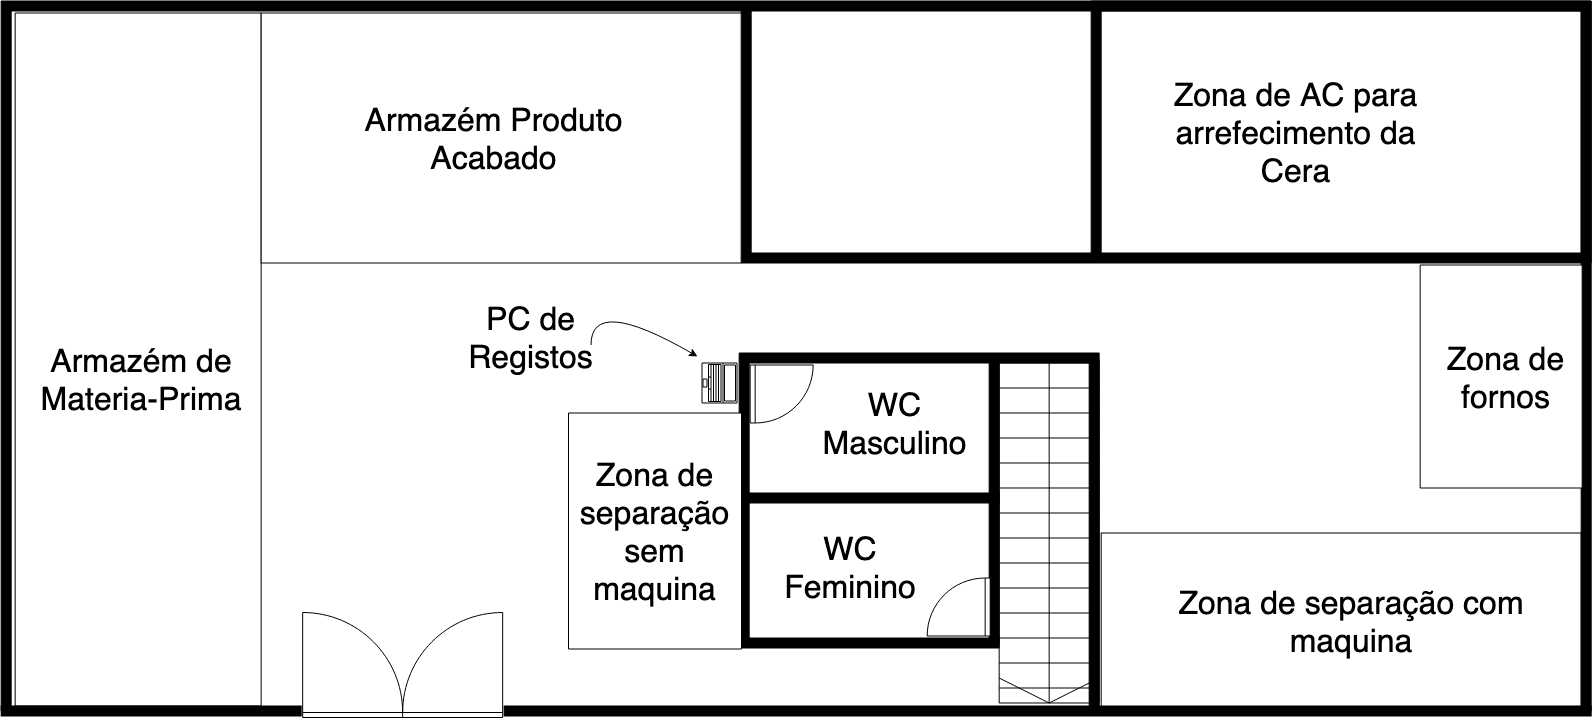
\includegraphics[width=\textwidth,keepaspectratio]{figuras/PlantaNaturalLife.png}
		\caption{Planta da fábrica}\label{fig:planta_naturallife} 
	\end{center}
\end{figure}

\noindent
Do lado esquerdo onde fica o armazém e onde é recepcionado a matéria-prima e do lado direito fica o espaço onde existe uma máquina que corta o corpo de plástico do círio. Após o corpo do círio, outro colaborador abre o corpo do círio e separa a cera do plástico. A alimentar a máquina está um operador que recebe o corpo do círio sem nenhum elemento metálico, tendo apenas que o colocar devidamente alinhado. Alguns círios, devido à sua forma, não podem ser processado nessa mesma máquina, tornando-se necessário que exista um ponto de separação manual, este fica no lado esquerdo da fábrica, junto à receção do material. Terminada a separação, a cera é levada para o forno. Quando esta termina de ser derretida é enformada e colocada num espaço de ar condicionado para arrefecer e solidificar. Normalmente este processo é feito ao fim do dia e durante a noite para poder aproveitar a baixa de temperatura ambiental.

\section{O Problema}
A recolha da informação era feito por meio de uma base de dados desenvolvida com o software Microsoft Access\label{sym:MS_ACCESS} com auxilio de alguns formulários embutidos na mesma. Aquilo que se previa ser uma solução temporária, acabou por se tornar definitiva pela simplicidade que a interface oferecia aos utilizadores, pela simples integração com outras aplicações Microsoft, como o Microsoft Excel\label{sym:MS_EXCEL} e Microsoft PowerBI\label{sym:MS_POWERBI}, e pela dificuldade de encontrar um sistema ERP\label{sym:ERP} comercial com as características da solução temporária, com um custo de aquisição que a empresa pudesse comportar e permitisse obter interfaces simplistas para os utilizadores que já se tinham acostumado com os formulários em Access.
No entanto a solução desenvolvida no Microsoft Access é bastante limitada, nomeadamente em executar o mesmo ficheiro em dois computadores ao mesmo tempo. Este constrangimento limita as opções da administração nos seus planos expansão da fábrica ou até fazer gestão da própria empresa durante o período laboral da empresa. Este é ainda o motivo que obriga os colaboradores a deslocar-se vários metros até ao computador para aí fazerem registos. Além do que já foi referido, ainda existe a limitação da base de dados não suportar níveis de acesso, o que quer dizer que qualquer pessoa com acesso ao computador poderá não só ver todos os registos da empresa como modificá-los ou até mesmo elimina-los. Assim, pretende-se com este projeto de estágio, a implementação de um novo sistema de recolha e consulta de informação, desenvolvido pelo estudante e consequente migração dos dados anteriormente registados.

\section{Estado da arte}
Existem varias ferramentas disponíveis para fazer a gestão dos recursos de uma empresa e cada uma com as suas características. Para analisar as opções disponíveis, selecionou-se alguns sistemas integrados de gestão empresarial (Enterprise Resource Planning - ERP) de forma a poder comparar os seus recursos com as necessidades da empresa. De seguida apresentam-se três das soluções estudadas.

\subsection{SAP ERP}
O SAP ERP é o produto principal da empresa alemã SAP AG, líder no segmento de software corporativos\cite{Wikipediab}. O SAP ERP é um sistema integrado de gestão empresarial transacional composto por vários tipos de módulos, cada um responsável por uma parte da atividade da empresa.


\subsection{PRIMAVERA Executive}
O PRIMAVERA Executive é um software ERP desenvolvido pela empresa PRIMAVERA Business Software Solutions com foco nas pequenas e médias empresas \cite{PRIMAVERABSS}. Trata-se de uma tecnológica portuguesa que se dedica ao desenvolvimento e comercialização de soluções de gestão e plataformas para integração de processos empresariais \cite{Wikipediaa}. Esta empresa afirmou-se no mercado nacional de soluções informáticas de gestão por ser pioneira no desenvolvimento de aplicações para Windows. \cite{Wikipediaa}.
As soluções ERP desta empresa contam ainda integração com os \textit{software}s de faturação da própria.

\subsection{Microsoft Dynamics}
Microsoft Dynamics é um pacote \textit{software} da Microsoft destinado a gestão corporativa ERP, para ajudar na tomada de decisão e melhoraria dos resultados administrativos e financeiros das empresas\cite{Wikipediac}.
Dentro deste pacote de \textit{software} existem as seguintes aplicações:
\begin{itemize}
	\item Dynamics 365 for Sales
	\item Dynamics 365 for Retail
	\item Dynamics 365 for Finance and Operations
	\item Dynamics 365 for Talent
\end{itemize}
Este pacote está disponível em várias edições nas quais varia as funcionalidades disponíveis de modo a se ajustar melhor às necessidades de cada empresa.

\newpage

\section{Comparação das opções disponíveis}
A informação coletada sobre as diferentes opções foi colocada na tabela \ref{tab:opcoes_mercado}

\begin{longtable}{|m{0.30\textwidth}|m{0.10\textwidth}|m{0.10\textwidth}|m{0.10\textwidth}|m{0.20\textwidth}|}
	\hline
	Característica & SAP & \specialcell{Primavera\\Executive} & \specialcell{Microsoft\\Dynamics} & Solução Própria\\ \hline
	Funções de gestão 
	de recursos da empresa		& \ding{51} & \ding{51} & \ding{51} & \ding{51}\\ \hline
	Acesso remoto externo		& \ding{51} & \ding{51} & \ding{51} & \ding{53}\\ \hline
	Suporte técnico de terceiros& \ding{51} & \ding{51} & \ding{51} & \ding{53}\\ \hline
	Controlo do desenvolvimento & \ding{53} & \ding{53} & \ding{53} & \ding{51}\\ \hline
	Atualizações do sistema		& \ding{51} & \ding{51} & \ding{51} & tem de as
																	desenvolver\\ \hline
	Adaptação total do sistema
	às necessidades da empresa	& \ding{53} & \ding{53} & \ding{53} & \ding{51}\\ \hline
	Implementação apenas dos recursos necessário
								& \ding{53} & \ding{53} & \ding{53} & \ding{51}\\ \hline
	Compatível com os planos de investimento a curto e médio prazo
								& \ding{53} & \ding{53} & \ding{53} & \ding{51}\\ \hline
	Curto período de adaptação dos utilizadores ao novo sistema
								& \ding{53} & \ding{53} & \ding{53} & \ding{51}\\ \hline
	\caption{Tabela resumo das opções de sistemas já desenvolvidos}
	\label{tab:opcoes_mercado}
\end{longtable}

No final desta analise, o caminho definido pela administração da Natural Life foi a criação de uma nova plataforma. Por esse motivo foi feita uma nova analise de opções à cerca do desenvolvimento da plataforma. Este documento foi entregue à administração para que o analisa-se e decidisse o modo como a aplicação deveria ser desenvolvida. O documento entregue esta presente no anexo \ref{anexo:A}. Desse documento foi extraída a tabela comparativa das opções para o desenvolvimento da plataforma. Esta é apresentada na tabela \ref{tab:opcoes_dev}.


\begin{longtable}{|p{0.20\textwidth}|p{0.15\textwidth}|p{0.25\textwidth}|p{0.25\textwidth}|}
	\hline
	& Opção                                                 & Vantagens                                                           & Desvantagens                                                                                        \\ \hline
	\multirow{6}{*}{Tipo de Aplicação}                                      & \multirow{3}{*}{Desktop}                              &                                                                     & Necessidade de configurar cada computador que receber a aplicação                                   \\
	&                                                       &                                                                     & Parar o computador para atualizar a aplicação                                                       \\
	&                                                       &                                                                     & Necessidade de um servidor de base de dados                                                         \\ \cline{2-4}
	& \multirow{3}{*}{Web}                                  & Acesso direto em qualquer computador                                & Necessidade de um servidor web e de base de dados                                                   \\
	&                                                       & Maior familiaridade com a plataforma por parte de programador       &                                                                                                     \\
	&                                                       & Menos pontos de falha                                               &                                                                                                     \\ \hline
	
	\multirow{5}{*}{Sistema Operativo}                                      & \multirow{3}{*}{Windows 10}                           & Familiaridade com o sistema                                         & Necessidade de comprar uma licença do Windows Server                                                \\
	&                                                       & Todas as máquinas já executam esta plataforma                       & Necessidade de aprender ASP.NET ou usar o XAMPP                                                     \\
	&                                                       &                                                                     & Se não for usado só software Microsoft não há garantias de segurança/ compatibilidade com o Windows \\ \cline{2-4} 
	& \multirow{2}{*}{Ubuntu 18.04}                         & Plataforma líder de mercado                                         & Curva de aprendizagem para manutenção básica                                                        \\
	&                                                       & Milhares de pacotes no repositório que são revisados pela Canonical &                                                                                                     \\ \hline
	
	\multirow{10}{*}{\specialcell{Sistema de Gestão\\de\\Base de Dados}}    & \multirow{3}{*}{\specialcell{Microsoft SQL\\Server}}  & Familiaridade com o software                                        & Versão Express limitada.                                                                            \\
	&                                                       & Versão Express gratuita                                             & Versões Enterprise e Standard pagas                                                                 \\
	&                                                       &                                                                     & Versão Developer não utilizável em produção                                                         \\ \cline{2-4}
	& \multirow{7}{*}{MariaDB}                              & Gratuito (versão Open Source)                                       & Não possui um ficheiro único para a base de dados.                                                  \\
	&                                                       & Totalmente compatível com MySQL da Oracle                           & Tem de ser instalado manualmente no Windows ou usado com recurso ao XAMPP                           \\
	&                                                       & Padrão no Ubuntu e no XAMPP                                         &                                                                                                     \\
	&                                                       & Escalável                                                           &                                                                                                     \\
	&                                                       & Fiável                                                              &                                                                                                     \\
	&                                                       & Recursos semelhante ao MS SQL Server                                &                                                                                                     \\
	&                                                       & Suporte nativo no Ubuntu                                            &                                                                                                     \\ \hline
	
	\multirow{5}{*}{Tipo de Máquina}                                        & \multirow{2}{*}{Real}                                 & Não dependência da operação de outras máquinas                      & Hardware dedicado                                                                                   \\
	&                                                       &                                                                     &                                                                                                     \\ \cline{2-4}
	& \multirow{3}{*}{Virtual}                              & Não necessita de hardware dedicado.                                 & Exige que o utilizador que esta a executar a VM nunca termine a sessão.                             \\
	&                                                       & Várias instâncias da máquina ao mesmo tempo.                        & Se a máquina real tiver de ser reiniciada, a VM tem de ser interrompida                             \\
	&                                                       & Backup muito fácil.                                                 & Partilha dos recursos da máquina hospedeira com a maquina virtual.                                  \\
	\hline
	\caption{Tabela resumo das opções para o desenvolvimento}
	\label{tab:opcoes_dev}
\end{longtable}


\section{Analise das opções disponíveis para o desenvolvimento do projeto}
O documento entregue incide sobre os aspetos base para a criação do sistema de informação: tipologia de aplicação, servidor, linguagens de programação, sistema de gestão de base de dados.\\
Primeiro definiu-se a tipologia de aplicação. Decidir sobre uma aplicação \textit{web} ou uma aplicação \textit{desktop} iria condicionar o trabalho futuro. Aqui a sugestão passou pelo desenvolvimento de uma aplicação \textit{web}, pois esta seria agnóstica de equipamento o que traria uma grande flexibilidade no futuro. Além deste fator, já se sabia que teria de existir uma servidor porque a base de dados seria  centralizada, logo não havia nenhum gasto extra com esta solução. Ficou desde logo decidido que seria o servidor seria uma máquina física com o sistema operativo Ubuntu 18.04\\
Ultrapassada esta fase, foram analisadas as linguagens de programação e optou-se pela linguagem PHP para o \textit{backend} e JavaScript para o \textit{frontend}. Ficou ainda decidido que de modo a tornar o desenvolvimento mais ágil e dar robustez ao serviço, devia ser utilizado o \textit{framework} Laravel. Esta escolha assentou no facto deste \textit{framework} já ser bastante utilizado, inclusivamente é tido como escolha de referência para projetos de missão crítica em PHP pelas suas características de segurança\cite{Mansuri2018}.\\
Por fim foi definido o sistema de gestão de base de dados (DataBase Management System - DBMS\label{sym:DBMS}). A opção opção recaiu sobre o Microsoft SQL Server apesar das vantagens enunciadas em relação ao MariaDB.\\
Dois pontos que não foi considerados neste documento foram o sistema e o serviço de \textit{versionamento}. A administração optou por deixar ao estudante das LES desde que o houvesse a garantia do repositório ser privado, uma vez que tirando o facto de assim ser esta opção em nada influenciava o sistema a ser implementado. Assim o sistema de versionamento escolhido foi o Git no serviço GitHub.

\section{Resumo final das opções tomadas para o desenvolvimento do projeto}
No final de todo este processo ficou decidido construir uma plataforma própria em formato de aplicação \textit{Web}. Esta aplicação web seria construida em PHP, com o framework Laravel, para o backend e JavaScript frontend. O sistema de gestão de base de dados escolhido foi o Microsoft SQL Server na edição Express e o servidor seria uma máquina física com o sistema operativo Ubuntu 18.04. Para fazer o versionamento do código foi utilizado um repositório privado no serviço GitHub.